%Vorlage fuer Thesen an der FFHS
\documentclass{../template/ffhsthesis}

\usepackage[utf8]{inputenc}

% addional configuration from sam
\usepackage{bibgerm}
\usepackage{hyperref}
\usepackage{cite}
\usepackage{etoolbox}
\usepackage{listings}
\usepackage{wrapfig}
\usepackage{fullpage}
\usepackage[section]{placeins}
\usepackage{float}%
\usepackage{verbatim}
\usepackage{filecontents}
\usepackage{siunitx}
\sisetup{per=slash, load=abbr}
\usepackage{tikz}
\usepackage{pgfplots}
\pgfplotsset{width=7cm,compat=newest}

\makeatother
\hypersetup{
    colorlinks = false,
    linkcolor = blue,
    urlcolor  = blue,
    citecolor = blue,
    anchorcolor = blue,
    pdfborder={0 0 0},
}
\setlength\parindent{0pt}




\begin{document}
% addional configuration from sam
\shorthandoff{"}
\renewcommand{\lstlistingname}{Codesequenz}


\lstset{literate=%
    {Ö}{{\"O}}1
    {Ä}{{\"A}}1
    {Ü}{{\"U}}1
    {ß}{{\ss}}1
    {ü}{{\"u}}1
    {ä}{{\"a}}1
    {ö}{{\"o}}1
    {~}{{\textasciitilde}}1
}




\lstdefinelanguage{C}
{
                basicstyle=\ttfamily\small,
                keywordstyle=\color{blue}\ttfamily,
                stringstyle=\color{red}\ttfamily,
                commentstyle=\color{green}\ttfamily,
                morecomment=[l][\color{magenta}]{\#}
}


\lstdefinelanguage
   [x64]{Assembler}     % add a "x64" dialect of Assembler
   [x86masm]{Assembler} % based on the "x86masm" dialect
   % with these extra keywords:
   {morekeywords={CDQE,CQO,CMPSQ,CMPXCHG16B,JRCXZ,LODSQ,MOVSXD, %
                  POPFQ,PUSHFQ,SCASQ,STOSQ,IRETQ,RDTSCP,SWAPGS, %
                  rax,rdx,rcx,rbx,rsi,rdi,rsp,rbp, %
                  r8,r8d,r8w,r8b,r9,r9d,r9w,r9b},
    basicstyle=\ttfamily\small,
    aboveskip={1.0\baselineskip},
    belowskip={1.0\baselineskip},
    columns=fixed,
    extendedchars=true,
    breaklines=true,
    tabsize=4,
    prebreak=\raisebox{0ex}[0ex][0ex]{\ensuremath{\hookleftarrow}},
    frame=single,
    showtabs=false,
    showspaces=false,
    showstringspaces=false,
    numbers=left,
    numberstyle=\small,
    stepnumber=1,
    captionpos=t,
	xleftmargin=0.5cm,
    numbersep=10pt} % etc.


\lstdefinelanguage{bash}
   % with these extra keywords:
   {
    basicstyle=\ttfamily\small,
    aboveskip={1.0\baselineskip},
    belowskip={1.0\baselineskip},
    columns=fixed,
    extendedchars=true,
    breaklines=true,
    tabsize=4,
    prebreak=\raisebox{0ex}[0ex][0ex]{\ensuremath{\hookleftarrow}},
    frame=single,
    showtabs=false,
    showspaces=false,
    showstringspaces=false,
    numbers=none,
    captionpos=t,
    numbersep=10pt}


\lstdefinelanguage{Ini}
{
    basicstyle=\ttfamily\small,
    columns=fullflexible,
    morecomment=[s][\color{blue}\bfseries]{[}{]},
    morecomment=[l]{\#},
    morecomment=[l]{;},
    commentstyle=\color{gray}\ttfamily,
    morekeywords={},
    otherkeywords={=,:},
    keywordstyle={\color{green}\bfseries}
}

\input{../template/custom-colors.tex}

\dokumentTyp{Bachelor-Thesis}
\studiengang{INF}
\title{Energie in der Informatik}
\subtitle{ durch bessere Software sparen ohne Verzicht} % optional
\titelbild[height=4.55cm,width=15cm]{images/Italy_Alps_and_Mediterranean.jpg}  % optional
\author{Samuel Riolo}
% \date{}
\wohnort{Kerzers}
%\referent{Name des Referenten\\ Titel\\Unterrichtetes Fach}
\referent{Jürg Hofer\\Dipl. El. Ing. ETH\\WING}
%\referent{Jürg Hofer\\ Titel\\Unterrichtetes Fach}
%\eingereichtBei{Prof.\ Dr.\ Martin Sutter\\Departement Informatik\\Departementsleiter} 


\maketitle

\begin{zusammenfassung}

Die Energiepolitik ist auf der ganzen Welt ein grosses Thema und wird heftig diskutiert. Immer mehr Leute sind der Überzeugung, dass eine Energiewende unumgänglich ist. Eines der wichtigsten Kriterien der Energiewende ist, dass Energie gespart wird. Dies kann sowohl durch die Senkung des Energieverbrauchs an sich als auch durch Optimierung der Produktion und Speicherung von Energie erreicht werden.
\par
Diese Arbeit befasst sich mit der Option, den Energieverbrauch zu senken. Es wird aufgezeigt, wo in der IT-Branche, speziell im Client- und Serverbereich, Potenzial besteht, Strom zu sparen.
\par
Im Rahmen der Arbeit wird eine Messmethode erforscht und entwickelt, um den Strombedarf eines CPU-Prozessors zu untersuchen. Damit kann dessen Energiebedarf pro Befehlssatz gemessen und analysiert werden. Die Untersuchung erfolgt auf zwei unterschiedlichen SoC-Board, nämlich eines mit RISC- und eines mit CISC-Architektur.

\textit{Todo: Einfügen der Resultat und Schlüsse, evtl. noch mehr zur Untersuchungsmethode (z.B. wie wird der Stromverbrauch gemessen?)}


\end{zusammenfassung}

\begin{abstract} 

-- Just an dirty Google translation as placeholder, I will fix it later --
\par
Energy policy is a big issue around the world and is hotly debated. More and more people are the
Believes that energy policy is unumgäglich. One of the main criteria of the energy transition, however, the
Energy is saved. This work will focus on a subsection of the energy transition. It should be pointed out,
where is the IT industry, especially in the client and server area, potential to save power. economic aspects
should be considered by the success in efficiency, without sacrificing the quality of the IT infrastructure
can be achieved.
\par
The work focused on it, the energy consumption per instruction set of a processor
analyze. It will be researched and developed a measurement methods to examine the current.....

\end{abstract}



\tableofcontents

\begin{abkuerzungen}[MUSTER] % Das Muster dient zur Bestimmung der Einrueckungstiefe
%\item[DInf] Departement Informatik
%\item[FFHS] Fernfachhochschule Schweiz
\item[SoC] System on Chip
\item[RISC] Reduced Instruction Set Computer
\item[CISC] Custom Instruction Set Computer
\item[ARM] Advanced RISC Machine
\item[EpI] Energy per Instruction
\item[TWh/a] $10^{12}$ Wattstunden oder $10^{9}$ Kilowattstunden pro Jahr
\item[ISR] Interrupt-Service-Routine
\item[RAM] Random-access memory


\end{abkuerzungen}


\startThesis % Befehl muss vor dem ersten chapter stehen (Seitennummerierung!)


% addional configuration from sam
\addtolength{\parskip}{\baselineskip}
\parindent 0pt 



% content
\chapter{Einleitung}

Die Energiepolitik ist auf der ganzen Welt ein grosses Thema und wird heftig diskutiert. Immer mehr Leute
sind der Überzeugung, dass eine Energiewende unumgäglich ist. Dabei wird die Energiewende von politischen, aber auch
von wirtschaftlichen Interessen beeinflusst. Die Energiewende beinhaltet aber nicht nur
das Produzieren von erneuerbaren Energien, sondern viele unterschiedliche Teilaspekte. Für die Energiewende
müssen Energieressourcen gespeichert werden, damit sie bei Bedarf genutzt werden können. Wird Strom über
Solaaranlagen in den Haushalten produziert, so muss die Energie ins Netz zurückfliessen. Dafür müssen
Hochspannungsleitungen so verändert werden, dass sie Strom in beide Richtungen fliessen lassen können.
Die heute verwendeten Energienanlagen, wie Windmühlen oder Solaaranlagen, produzieren in Europa so starke
Schwankungen, dass die Gefahr eines riesigen Blackouts besteht.
\par
Viele Probleme müssen für die Energiewende gelöst werden. Eines der wichtigsten Kriterien der Energiewende ist aber,
das Energie gespart wird. Diese Arbeit wird sich mit einem Teilgebiet der Energiewende befassen.
Es soll aufgezeigt werden, wo in der IT-Branche, speziell im Client- und Serverbereich, Potenzial besteht,
Strom zu sparen. Auch gerade deswegen, weil die IT-Branche von einem enormen Wachstum geprägt ist. Wirtschaftliche Aspekte sollen
berücksichtigt werden, indem der Erfolg des Stromsparens ohne Verzicht auf die Qualität der IT-Infrastruktur erzielt
werden kann. 
\par
Ein Computer ist ein Gerät, dessen Besonderheit darin besteht, dass es durch logische und arithmetische Befehle programmiert
werden kann. In andere Worte gefasst, heisst das, dass die Software die Hardware ansteuert und die Hardware Befehl um Befehl ausführt.
Genau dieser Aspekt soll in der Arbeit abgehandelt werden. Es soll eine Basis gebildet werden, die aufzeigt, wie man durch bessere Software Strom
sparen kann. Die Arbeit wird sich darauf konzentrieren, den Energiebedarf pro Befehlssatz eines Prozessors zu analysieren.
Es soll eine Messmethoden erforscht und entwickelt werden, um den Strombedarf eines CPU zu untersuchen. Die Untersuchung soll
auf unterschiedlichen SoC (System on Chip) Architekturen erfolgen, damit Vergleiche erstellt werden können.
\par
Ziel der Arbeit ist es, Daten zu erhalten, die Informationen über den Energieverbrauch einzelner Befehlssätze liefern. Diese Daten
könnte man zum Beispiel auf Workstations oder Server hochrechnen. Für CPU-Befehle, die sich eher verschwenderisch auf den
Strombedarf auswirken, könnte man Alternativen finden. Man könnte sich zum Beispiel eine Green-Flag für den GNU C Compiler
vorstellen, der "grünen Maschinencode" erstellt.



% Denn nur so kann eine Aussage gemacht werden, ob ein neues System auch zielführend ist. Erst im zweiten Schritt können dann
% Ansätze evaluiert werden, die zum Ziel der Reduktion des Energieverbrauchs dienen können. 
% Dabei sollen unterschiedliche Schichten der Software analysiert werden. Es sollen Antworten auf die folgenden Fragen gefunden werden:
% Wie kann das Betriebsystem Strom sparen; ist es möglich durch bessere Treiber die Hardware auf Standby zu setzen, wenn sie nicht gebraucht wird
% oder kann bereits beim Kompilieren effizenter gearbeitet werden. Am Schluss soll geprüft werden,
% ob die Ansätze in der Realität anwendbar und wirtschaflich interessant sind. Es sollen konkrete Beispiele enstehen, wo und wie ein
% IT-Betrieb Stromersparnisse erzielen kann.




\chapter{Energiepolitik 2050}

\section{Energiepolitische Entscheidungen in der Schweiz}
Durch den Beschluss am 2011 des Bundesrat und Parlament wurde ein Grundsatzentscheid getroffen,
schrittweise aus der Kernenergie auszusteigen\cite{bfe_energiestrategie}. 
\par
Die Stillegung der fünf Kernkraftwerke in der Schweiz, sollen am Ende ihrer sicherheitstechnischen
Betriebsdauer erfolgen. Diese Entscheidung und insbesondere auch die internationale Veränderungen 
im der Energieversorgung bewirkt eine starke Wende in das schweizerische Energieumfeld.
Am 4. September 2013 wurde vom Bundesrat und Parlament das erste Massnahmenpaket verabschiedet, um
die Sicherheit der Energieversorgung in der Schweiz zu garantieren. Das Massnahmenpaket setzt in erster
Line auf eine ausgewogene Ausschöpfung der vorhandene Potenziale der Wasserkraft und der neuen erneuerbaren
Energien. Am 8. Dezember 2014 wurde das Massnahmenpaket vom Nationalrat und am 23. September 2015 vom Ständerat
angenommen. Differenzen werden zur Zeit zwischen den Räten bereinigt bevor diese nochmals über die
gesamte Vorlage abstimmt. 
\par
Das Parlament hat bereits mit einer Gesetzesänderung (pa.lv. 12.400) verabschiedet, dass am Anfang 2014 in
Kraft getreten ist. Dadurch werden der Ausbau der erneuerbaren Energien gefördert. Auch beinhaltet
diese Gesetzesänderung ein Aktionsplan für eine stärkere Energieforschung.

\section{Stromnachfrage 2010 - 2050}

Die Prognosen der Stromnachfrage über ein Zeithorizont von 40 Jahren ist generell sehr schwer\cite{eth_energiezukunft_schweiz}.
Dennoch bilden sich plausible Wert für das Jahr 2050 ab. Dabei werden die Parameter Bevölkerungswachstum,
Pro-Kopf-Einkommen und Stromintensität aufgrund der Trends, berücksichtigt.
\par
Heute geht man von einem Stromverbrauch von 63 TWh pro Jahr aus (inkl. Netzverluste von etwa 7\% aber
ohne Speicherpumpenverluste). Für das Jahr 2050 geht man davon aus, dass sich die Extremwerte von
60 TWh/a bis über 100TWh/a abzeichnen werden.
\par
Der schrittweise Ausstieg aus der Atomkraft und gleichzeitig die neuen Ansprüche des Strombedarfs abzudecken,
scheint für das 2050 schwierig aber nicht unmöglich zu sein. Die Transformation des Energiesystem in einem
Zeithorizont von mehrere Jahrzehnten ist im Grundsatz technologisch machbar und wirtschaftlich verkraftbar.
Für den Erfolg muss in die Forschung und Einsatz von Photovoltaik, Biomasse, Wind und Geothermie investiert werden.
Auch der Ausbau von Stauseen, als Pumpspeicherkraftwerken wird dafür nötig sein.
\par
Die CO\textsubscript{2}-Reduzierung und die damit kombinierte Stromerzeugung aus erneuerbare Energien, führt auch dazu,
dass die importiert mengen um 65\% reduziert werden. Dabei wird ein wesentlicher Beitrag geleistet, dass die Schweiz
hinsichtlich der Stromversorgung unabhängiger wird und eine besser  Versorgungssicherheit des Landes gewährleistet wird.
 



\section{}








\chapter{Stand des Wissens und der Technik}
\section{Funktionsweise eines Prozessors}

Ein Prozessor ist eine universelle Rechnermaschine, die sich durch eine definierte Reihe von Anweisungen programmieren lässt. Zu den arithmetischen Anweisungen gehören der Zugriff auf Speicheradressen und Sprünge innerhalb der Abfolge der Anweisungen.
Bereits der britische Mathematiker Alan Turing konnte aufzeigen, dass ein universelles Berechnungsmodell möglich ist, wenn ein Rechner neben Speicherzugriff auch Sprünge besitzt\cite{Hoffmann2014l}. Auf diesen besonderen Eigenschaften bauen die heutigen Prozessoren auf. Ein Programm, das den Prozessor ansteuert, besteht aus einer endlichen Anzahl von geordneten Anweisungen. Der Prozessor befolgt, streng nach dem Ablauf, Anweisung für Anweisung, die auch Sprünge zu anderen Stellen innerhalb des Programms besitzen.
\par
Die Prozessoren, auch Zentraleinheiten oder CPUs genannt, besitzen im Inneren drei Einheiten, die über einen Datenbus verbunden sind. Dies ist in der \autoref{fig:CPU} ersichtlich. Dabei kann der Datenbus je nach Grösse oder Leistung des CPUs variieren. Die meist verbreiteten CPUs, die in den heutigen PC verbaut sind, haben einen 64bit-Datenbus. In dieser Arbeit wird aber mit kleineren CPUs gearbeitet, die einen 32bit-Datenbus besitzen. Die Control Unit\cite{patterson2013computer} ist dafür verantwortlich, dass das Programm immer an der richtigen Stelle ausgeführt wird. Sie nimmt Anweisungen an, dekodiert diese und übergibt sie der ALU. Die Übergabe der Daten an die ALU und die Register erfolgt durch die Weichenstellung des Datenbusses. Die Arithmetic and Logical Unit (ALU) ermöglicht es, Rechenoperationen sowie logische Operationen an den Daten auszuführen. Die Register haben die Grösse des Datenbusses und dienen dazu, die Daten von und zur ALU zu bewegen. Eine CPU besitzt mehrere Register, die je nach CPU-Architektur variieren. Die Register lassen sich in zwei Kategorien, Universal- und Hilfsregister, unterteilen. In den Universalregistern lassen sich die zu bearbeitenden Daten speichern. Die Hilfsregister haben eine besondere Rolle zugeordnet erhalten. Beispielsweise zählt das Statusregister zu den Hilfsregistern. Dieses spezielle Hilfsregister gibt Aufschluss über das Resultat der vorherigen Operation. So lässt sich über dieses Hilfsregisters herauslesen, ob eine Operation von zwei Zahlen den möglichen Speicherplatz des Registers übersteigt und es zu einem sogenannten "overflow" kommt.
Da die Anzahl meist sehr klein ist, müssen die Daten immer wieder von den Registern in den RAM und wieder zurückgeladen werden.
\par
Prozessoren sind als elektronische Schaltkreise realisiert. Die Schaltkreise werden durch die Halbleitertechnologie hergestellt. Die Millionen von witzigen Transistoren, die ein Prozessor beinhaltet, werden zu logischen Bausteinen verdrahtet.
\par
In dieser Arbeit ist die Funktionsweise der ALU relevant. Wir wissen, dass die ALU eine Reihe von Anweisungen erhält und somit jeden erdenklichen Algorithmus ausführen kann. Im Rahmen dieser Arbeit wird eine Methode entwickelt, um den Energieverbrauch einer einzelnen Anweisung der ALU messen können.



\begin{figure}[t]
\centering
\includegraphics[width=1.0\textwidth]{images/cpu.pdf}
\caption{Central Processing Unit}
\label{fig:CPU}
\end{figure}

\section{Aufbau des Linux Betriebssystem}
Durch die Inspiration des Betriebssystem Minix, das von Andrew S. Tanenbaum für Ausbildungszwecke erstellt wurde, machte sich Linus Torvalds zum Ziel ein vollwertiges System neu zu schreiben. Im Jahr 1991 erschien die erste Linux Version 0.01\cite{ehses2011systemprogrammierung_chap2}. Heute ist es ein weit verbreitetes Betriebssystem, dass im Bereich Desktop, Server, Smartphone und Embedded Systems angewendet wird.
\par
Die Aufgabe des Betriebssystemkern, der meistens nur einfach Kernel genannt wird, ist es eine Softwareschicht zwischen Hardware und Programme zu erstellen. Jedes Programm hat somit nicht ein direkten Zugriff auf die Hardware. Jedes Programm, dass Informationen der Hardware benötigt muss durch die Schicht des Kernels gehen. Die Kommunikation die durch Programm und Kernel besteht, werden Systemaufrufe (engl. Systemcalls) genannt. Die unterschiedlichen Systemaufrufe sind im POSIX standardisiert\cite{ehses2011systemprogrammierung_chap2}. Zusätzlich erstellt der Kernel eine Art Abkapselung eines Programms. Dadurch können mehrere Programme gleichzeitig laufen ohne dass das eine Programm zugriff auf das andere hat. Der Kernel Verteilt die freien Ressourcen des CPU abwechslungsweise an die Programme. Dieses Verfahren heisst Multitasking und wurde seit den Anfängen unterstützt.
\par
Durch die Zusätzliche Softwareschicht der der Kernel bietet, müssen Programmierer ein Programm nicht für eine bestimmte Hardware schreiben, sondern für ein bestimmtes Betriebssystem. Dies ermöglicht eine höhere Portabilität eines Programm. Hardware wie Festplatten oder Netzwerkcontroller werden vom Kernel vereinheitlicht und dem Programm durch Systemaufrufe zur Verfügung gestellt.
\par

\begin{wrapfigure}{L}{0.49\textwidth}
\centering
\includegraphics[scale=0.8]{images/kernel.pdf}
\caption{Linux Kernel}
\label{fig:kernel}
\end{wrapfigure}

Die \autoref{fig:kernel} zeigt wie die Unterschiedlichen Schichten miteinander kommunizieren. Eine Anwendung wird ausschliesslich im Benutzermodus(engl. User Space) ausgeführt. Durch Systemaufrufe werden anfragen an den Kernel geleitet. Dabei findet ein Kontextwechsel statt vom unprivilegierter in den privilegierten Modus. Der unprivilegierter Modus bezeichnet den Benutzermodus in dem eine Applikation nur beschränkte Verfügbarkeit des Arbeitsspeicher und CPU Befehlssätze hat. Dies stellt sicher das eine Applikation gegenüber des Rest des System Abgekapselt betreiben wird und nicht ausbrechen kann. Nach dem Systemaufruf geht der Prozessor in den privilegierten Modus rüber und der Kernel trägt die Verantwortung die Anfrage im Kernelmodus (engl. Kernel Space) zu verarbeiten. Der Kernelmodus hat im Gegensatz zum Benutzermodus keine Einschränkungen und hat deswegen auch Zugang zur Hardware und Arbeitsspeicher. Der Kontextwechsel dient also dazu dass Programmcode der nicht zum Kernel gehört nur in einem unprivilegierten Modus ausgeführt werden kann.


\section{Unterschiede CISC und RISC CPUs}

Die Instruktionsarchitekturen der CPUs kann in zwei Gruppen unterteilt werden. Die CISC-Prozessoren (Custom Instruction Set Computer) mit sehr komplex und umfangreiche Instruktionsanweisungen und die RISC-Prozessoren (Reduced Instruction Set Computer) mit sehr primitive Instruktionsanweisungen.
\par
Der x86-Befehlssatz wurde durch den Intel 8086 Prozessor 1978 eingeführt und wurde somit zum Urvater moderne CISC-Prozessoren. Schon damals besitze dieser Prozessor ca. 120 Befehlssätze. Im Verlauf der Jahren zeichneten sich die CISC-Prozessoren mit immer mehr und komplexeren Befehlssätze aus. Dabei wurde immer beachtet das die Architektur, der neueren Modelle Rückwärtskompatibel, damit die Software ohne Anpassung auf neueren Prozessoren laufen kann. Die CISC-Architektur erlaubt es komplexe Instruktionen in einem Befehlssatz zu schreiben. Dabei wird der Befehlssatz von der CPU dekodiert und in einem oder mehreren Taktzyklen ausgeführt. Die Komplexität der Befehlssätze geht so weit das sogar Hardwareschleifen möglich werden. Ein anderes Merkmal der CISC-Prozessoren ist die geringe Anzahl der Register. Dafür kann ein Befehlssatz direkt die Anweisung haben, Daten von einer Speicherzelle im RAM zu einer andere zu transferiert ohne dabei auf ein Register angewiesen zu sein. Damit die immer komplexeren Befehlssätze dekodiert und in Instruktionen aufgeteilt werden können, besitzen die heutige CISC-Prozessoren sehr umfassende Steuerwerke. Allerdings bestehen die Steuerwerke nicht nur als Hardware Implementation, sondern besitzen teils innerhalb Microcode, die die Instruktionen an die ALU (Rechnerwerk) bilden kann.
\par






\section{Energy Storage in a Capacitor}


Grundlage Technische Informatik Kap. Halbleitertechnik lesen!


%Table 1.2. Double-precision VFP operations
%Instruction types	Issue latency
%DP MUL and MAC	2 cycle
%SP DIV, SQRT	14 cycles
%DP DIV, SQRT	28 cycles
%All other instructions	1 cycle


\chapter{Idee und Zielsetzung}


\chapter{Aufbau des Experiments}

In diesem Kapitel wird die Methode beschrieben, die zur Messung des Energieverbrauchs eines Befehlssatz verwendet wird. Es wird aufgezeigt, welche Schritte im Rahmen der Messung vollzogen werden. Dabei wird auf die einzelnen technischen Elemente eingegangen, die zur Umsetzung des Experiments erforderlich sind. 
\section{Auswahl und Beschreibung der Messmethode}
\label{chap:auswahl_beschreibung_methode}

Während die CPU ein Programm ausführt, das aus einer Reihe von Befehlssätzen besteht, verbraucht sie unterschiedlich viel Strom. Die Idee der hier erstellten Messmethode ist es, ein Programm kontrolliert und mit präzis ausgewählten Befehlssätzen auf der CPU durchlaufen zu lassen. Das Programm in Form eines Benchmarks ist so konzipiert, dass ein bestimmter Befehlssatz millionenfach wiederholt wird. Dadurch wird der Stromverbrauch während der Ausführung über einen längeren Zeitraum konstant gehalten. Denn nur so ist eine aussagekräftige Messung möglich, da ein einzelner Befehlssatz so schnell durchläuft, dass er kaum messbar ist. Da die Ausführung der Befehlssätze wiederholt wird, muss die Messung durch die Anzahl der ausgeführten Wiederholungen geteilt werden.
\par
Die Strommessung erfolgt vom Leistungsverbrauch des ganzen Gerätes. Optimal wäre es, nur die Leistung der CPU zu messen. Dafür müsste aber die CPU vom Board ausgelötet und eine speziell dafür gebaute Messvorrichtung verwendet werden. Dazu kommt, dass nicht alle Datenblätter, welche die erforderliche Beschreibung und Belegung der Pins enthalten, für jedes Board oder für jeden Chip verfügbar sind. Deshalb wird ein SoC eingesetzt und die gesamte Leistung gemessen. SoC sind verfügbar auf kleinen Entwickler-Boards, die keine Lüfter, Laufwerke oder andere Verbraucher aufweisen, die hinsichtlich der Leistung störende Unregelmässigkeiten verursachen würden.



\begin{wrapfigure}{R}{0.6\textwidth}
\centering
\includegraphics[scale=0.5]{images/schema.pdf}
\caption{Elektroschema für die Messung}
\label{fig:Elektroschema}
\end{wrapfigure}


Die für diese Arbeit verwendeten Boards werden im nächsten Kapitel im \autoref{beschreibung_hardware} beschrieben. Es wird davon ausgegangen, dass die Komponenten auf dem Board, abgesehen vom CPU selbst, während der Durchführung des Benchmarks vernachlässigbar kleine Leistungsschwankungen aufweisen. Die Messung erhält somit lediglich die Grundleistung der CPU, die vom Resultat abgezogen werden muss. Die Speisung erfolgt über einen Spannungsregler, der der Schaltung eine konstante Spannung liefert. Zwischen dem Spannungsregler und der Schaltung ist ein Amperemeter (Multimeter) zwischengeschaltet, der die Messung vornimmt. In der Abbildung \ref{fig:Elektroschema} ist das Elektroschema und die Platzierung des Amperemeters ersichtlich.
\par
Der eigentliche Kern des Benchmarks besteht aus gezielten und kurzen Assembler-Zeilen. Der Assemblercode bewirkt eine Schleife über einen zu testenden Befehlssatz. Damit das Ergebnis über einen längeren Zeitraum gemessen werden kann, wird der zu testende Befehlssatz einige Milliarden Mal  wiederholt. So wird ein Zeitraum von zirka zwei bis drei Minuten erzeugt, in welchem die Messung auf einem 800MHz CISC-Prozessor vorgenommen werden kann.
\par
Während dem Durchlaufen des Benchmarks darf die Ausführung nicht gestört werden. Jedes moderne Betriebssystem ist multitaskingfähig. Das bedeutet, dass das Betriebssystem eine Zeitscheibe besitzt und die Ressourcen der CPU abwechslungsweise an die Prozesse verteilt werden. Ein Benchmark darf also nicht als gewöhnlicher Prozess von einem Betriebssystem gestartet werden. Würde man das tun, hätte man keine Kontrolle, wann und wie viele Ressourcen der Benchmark schliesslich zugesprochen bekommt. Diese mangelnde Kontrolle würde das Messresultat verfälschen. Im Rahmen dieser Arbeit musste daher eine Methode erarbeitet werden, bei der der Benchmark während der Durchführung die vollen Ressourcen der CPU zugeteilt erhält und somit ein kontrollierter Ablauf garantiert ist.
\par
Die Ursprungsidee war es, direkt auf Baremetal zu arbeiten. Baremetal ist eine Ausdruck dafür, dass direkt auf der Hardware gearbeitet wird. Bei dieser Methode wird auf ein Betriebssystem verzichtet. Nach dem Bootprozess der Hardware wird ein Programm direkt gestartet und ausgeführt. An dieser Stelle wäre der Benchmark zum Zug gekommen. Eine speziell dafür präparierte Partition bootet die Hardware und führt den Benchmark aus.
\par
Für die Baremetal-Methode wurde ein funktionstüchtiger Prototyp erstellt. Es zeigten sich aber einige Nachteile. Auf komplexerer Hardware mit x86-Prozessoren ist der Boot-Vorgang um ein Vielfaches aufwendiger\cite{intel_boot_process}. Diese Prozessoren-Typen können nicht einfach beim Einschalten einen Programmcode ausführen. Es muss vorher eine lange Reihe von Abläufen in der Preboot Phase berücksichtigt und ausgeführt werden. Ein weiterer Nachteil der Baremetal-Methode ist die Überprüfung des Benchmarks. Die Gewährleistung, dass der Benchmark erwartungsgemäss funktioniert beziehungsweise überhaupt ausgeführt wird, benötigt ein Feedback nach aussen. Eine LED-Leuchte würde für dieses Feedback bereits ausreichen. Allerdings sind die GPIOs, die benötigt werden, um das LED zu steuern, je nach SoC sehr schwer anzusprechen, weil sie über einen PCI-Bus verbunden sind. Normalerweise stellt das Betriebssystem die nötigen C-Libraries zur Verfügung, um Komponenten, wie die GPIO, über einen PCI-Bus anzusteuern. Dieses fehlt hier jedoch gerade. Negativ wirkt sich zusätzlich die aufwendige Vorbereitung jedes einzelnen Tests aus. Für jeden Test muss eine Partition mit dem Benchmark erstellt und auf ein Medium kopiert werden. Damit die Messung erfolgen kann, muss dabei auch jedes Mal die Hardware neu gestartet werden. Unter diesen Umständen wird ein automatisierter Betrieb erheblich erschwert.
\par
Wegen der oben genannten Nachteile, wurde ein neues Konzept ausgearbeitet. Das neue Konzept arbeitet auf dem Betriebssystem Linux und bringt dadurch dessen Vorteile mit sich. Es muss sichergestellt werden, dass der Benchmark ohne Unterbrüche und abgeschirmt von anderen Prozessen durchgeführt wird. Um dies zu erreichen, wird der Benchmark anstatt im Benutzermodus (engl. User Space) im Kernelmodus (engl. Kernel Space) ausgeführt\cite{Mandl2010}. Der Programmcode, der innerhalb des Kernelmodus ausgeführt wird, muss als Kernelmodul kompiliert und im Kernel angemeldet werden. Schliesslich kann nur ein Interrupt den Code im Kernelmodul ausführen. Die genaue Beschreibung wird nachfolgend im \autoref{chap:benchmark_basis_interrupts} erläutert. Durch die Vornahme des Benchmarks im Kernelmodul werden alle Prozesse, die auf dem Betriebssystem parallel laufen, gestoppt und der Benchmark bekommt die vollen CPU-Ressourcen zugesprochen. In ein Kernelmodul können unterschiedliche Benchmarks gleichzeitig hinein kompiliert werden. Somit wird die Ausführung unterschiedlicher Tests vereinfacht. Dadurch wird eine spätere Automatisation ermöglicht, was zu einer Erleichterung der Messung beiträgt. 

 



 

\section{Beschreibung der Hardware}
\label{beschreibung_hardware}
\subsection{Intel Galileo Gen2}

\begin{wrapfigure}{r}{0.6\textwidth}
\centering
\includegraphics[scale=0.5]{images/iot_galileo.png}
\caption{Intel Galileo Gen2\cite{intel_galileo_image}}
\label{fig:Intel Galileo Gen2}
\end{wrapfigure}

Das Galileo Developer Board\cite{intel_datasheet_galileo} der zweiten Generation von
Intel ist ein SoC und besitzt einen Intel® Quark™ SoC X1000 Prozessor. Die Architektur des 32bit Prozessor basiert auf x86\cite{intel_datasheet} und somit ist das Galileo
Board eines der Wenigen, auf denen ein CISC-Prozessor verbaut wurde. Die Hardware
besitzt keinen Videoausgang. Es ist also nur möglich, über eine RS232 Schnittstelle oder über Ethernet,
eine Verbindung zum System zu erstellen. Die GPIO Ein- und Ausgänge sind über den
PCI-Bus verbunden. Somit ist es sehr schwer, ohne passender Treiber oder
Softwareschicht die GPIO anzusprechen. Im Vergleich sind die GPIO des RaspberryPI, das als zweites Board gewählt wurde,
direkt über eine Speicheradresse ansprechbar.
\par
Von Intel wird ein angepasstes Betriebssystem als fixfertiges Image angeboten. Dieses System basiert auf
der Linux Distribution Yocto. Es sind aber auch inoffizielle Debian Distributionen im
Internet erhältlich. Der Vorteil von Debian gegenüber der offiziellen Version, ist die
grössere Verbreitung und die damit verbundenen Hilfestellungen im Internet. Das Cross-Compiling eines Kernelmoduls scheint so einfacher als auf der Yocto-Distribution.


\subsection{RaspberryPi}


\begin{wrapfigure}{r}{0.6\textwidth}
\centering
\includegraphics[scale=0.4]{images/raspberry-pi-2.png}
\caption{Raspberry Pi 1 A\cite{raspberry_image}}
\label{fig:Raspberry Pi 1 A}
\end{wrapfigure}


Als zweites Experimentier-Board wird das Raspberry Pi Model B\cite{raspberry_foundation} verwendet. Das Board wird von der Raspberry Pi Foundation betrieben. Das Modell besitzt einen Broadcom BCM2835\cite{broadcom_datasheet} Chip. Der darin verbaute Prozessor wurde von der Firma ARM unter dem Namen ARM1176JZFS\cite{arm_datasheet} (ARM11) spezifiziert. Die Software muss für die Architektur ARMv6 kompiliert werden. Im Gegensatz zum Galileo Board von Intel ist der Prozessor ein RISC-CPU. Beide Boards haben eine 32bit Adressierung.
\par
Eine Remote-Verbindung lässt sich über eine serielle-Schnittstelle oder über Ethernet realisieren. Durch das Vorhandensein eines Videoausgangs und eines USB-Anschlusses, würde sich das Raspberry Pi auch direkt über Monitor und Tastatur bedienen lassen. Die GPIOs sind direkt über die Speicheradressierung ansprechbar. Somit wäre eine Erweiterung des Benchmarks, der in Assembler geschrieben ist, durchaus denkbar. So könnten auf einfache Weise weitere Messungen über die GPIO erfolgen. Das offizielle Betriebssystem der Foundation ist ein Debian basiertes OS mit dem Name Raspbian. Zusätzlich werden als Third-Party Produkte weitere unterschiedliche Betriebssysteme zur Verfügung gestellt. 













\section{Benchmark auf Basis von Interrupts}
\label{chap:benchmark_basis_interrupts}

% A system call is a request in a Unix-like operating
% system made via a software interrupt by 
% Found on http://www.linfo.org/software_interrupt.html


Der Aufbau der Messmethode basiert auf Softwareinterrupts. Dafür wurde ein eigener Kernelmodul erstellt, der den Benchmark beinhaltet und auf verlangen ausführt.
\par
Ein Interrupt erzwingt den Linux Kernel vom Benutzermodus in den Kernelmodus zu wechseln\cite{Mandl2010_3}. Beim Wechsel werden alle laufende Prozesse zwischen gespeichert, angehalten und anschliessend wird eine Interrupt-Service-Routine (ISR) aufgerufen. Genau diese Eigenschaft wird für den Aufbau der Messmethode verwendet. Den während der Ausführung des ISR sind alle Prozesse angehalten und können der Benchmark der sich selbst in der ISR befindet nicht unterbrechen. Somit wird sicher gestellt das nur der Benchmark ausgeführt und die volle Ressourcen des CPU bekommt bis er fertig ist.
\par
Interrupts sind dafür gemacht, damit sie sofort verarbeitet werden. Ein kleines Beispiel soll dies veranschaulichen. Der Benutzer eines Computer drückt eine Taste auf der Tastatur. Dadurch produziert er ein Hardware-Interrupt. Der aktuelle Prozess wird gespeichert und angehalten. Der Kernel stellt über eine Vektor-Tabelle fest um welchen Interrupt es sich handelt und führt die passende ISR aus, die zur Verarbeitung der gedrückte Tasten dient. ISR sind sehr kurze Programmcodes (Microcode). In diesem Fall speichert der Programmcode die gedrückte Taste in den RAM und übergibt die Ressourcen wieder frei. Der letzte Prozess wird danach, falls er nicht bereits fertig war, weitergeführt. Die Interrupts sind nötig um die Daten am Zeitpunkt des Geschehens zu verarbeiten.
\par
\autoref{fig:Interrupt} beschreibt die unterschiedlichen Interrupts und der Ablauf nach einem eingehender Interrupt. Die Hardware-Interrupts\footnote{Je nach Literatur, Sprache oder Betriebssystem werden unterschiedliche Fachausdrücke verwendet. Der Kontext bleibt aber der selbe.} wurden bereits oben beschrieben. Die "Exception / Trap" sind Interrupts die der CPU selber produziert. Als Beispiel für ein solches Interrupt wäre "Divisions by Zero", wenn man probiert eine Zahl durch Null zu teilen. Die Messmethode in dieser Arbeit stützt sich auf die Software-Interrupts. Software-Interrupts werden häufig verwendet um durch ein Kontextwechsel eine Aufgabe dem Kernel zu übergeben. Durch den Kontextwechsel wird vom unprivilegierten Ring  (Benutzermodus) in den privilegierten Ring (Kernelmodus) gewechselt. Dadurch können auf Befehlssätze und Speicheradressen zugegriffen die im Benutzermodus nicht möglich wären ohne unsicheren Code ausführen zu müssen. Dies wird zum Beispiel notwendig wenn man ein File lesen möchte.

Todo

\begin{figure}[H]
\centering
\includegraphics[width=1.0\textwidth]{images/interrupt_ea.pdf}
\caption{Interrupt}
\label{fig:Interrupt}
\end{figure}

\section{Starten des Benchmark über procfs}

Der Benchmark wurde in Form eines Kernelmodul für ein Linux Betriebssystem gebaut. Das Kernelmodul registriert für jeden Benchmark ein Pseudofile, das unter der Verzeichnisstruktur \texttt{/proc/benchmark/} abrufbar ist.
\par
Das \texttt{procfs} oder \texttt{proc filesystem} genannter Filesystem erstellt eine Schnittstelle zwischen dem Benutzermodus und dem Kernelmodus. Es ist ein virtuelles Filesystem, dass unter der Verzeichnisstruktur \texttt{/proc} gemountet wurde\cite{mauerer2010professional}. Die Dateien die sich darin befinden sind Pseudofiles. Sie sind virtuelle, weil sie nicht wirklich existieren und somit auch nicht auf ein Medium gespeichert sind. Beim schreiben beziehungsweise lesen werden die Information am Kernel weiter gegeben, verarbeitet und zurück zum lesen gestellt. Weil das verhalten der Schnittstelle einer Datei entspricht, können für die Lese- und Schreiboperation, die Linux Standart-Werkzeuge verwendet werden.

\lstset{language=Bash}
\begin{lstlisting}
sriolo@desktop ~ $ cat /proc/uptime 
571433.06 1229766.89
\end{lstlisting}
\begin{lstlisting}
sriolo@desktop ~ $ echo 1 > /proc/sys/net/ipv4/conf/default/forwarding
\end{lstlisting}

Im ersten Beispiel wird aus der Datei \texttt{uptime} gelesen, die Betriebszeit kommt als Ausgabe. Das folgende zweite Beispiel zeigt wie in einer Datei geschrieben werden kann. Dabei wird Kernel mitgeteilt dass, er das IP-Forwarding einschalten soll. Ein ähnlicher Aufbau hat das \texttt{sys filesystem}. Die Kommunikation ist dabei schwieriger weil das Design nicht für Menschen lesbar ist, sondern für Programme im Benutzermodus. Im Gegensatz dazu kann das \texttt{procfs} mit den Standard-Werkzeuge im ASCII-Format gelesen und geschrieben werden.
\par
Das \texttt{procfs} ist an dieser Stelle wichtig, weil der Benchmark im Kernelmodus laufen muss. Durch den Befehl \texttt{cat} auf die entsprechende Datei des Benchmark, startet im Kernelmodus den Ablauf für die Messung und gibt die verwendete Zeit als Ausgabe an. Das folgende Beispiel zeigt wie der Benchmark gestartet wird und der CPU durch eine Addieroperation ausgelastet wird.

\begin{lstlisting}
root@galileo ~ $ cat /proc/benchmark/addl_32
321
\end{lstlisting}


\section{Aufbau der Software für die Messung}

Der Grundbau der Software wurde mit der Programmiersprache C geschrieben. Der Kern des Benchmark besteht aus wenige Assembler Befehlssätze. Der Kernelmodul beinhaltet alle in dieser Arbeit relevante Benchmarks. 






\begin{figure}[H]
\centering
\includegraphics[width=1.0\textwidth]{images/benchmark_ea.pdf}
\caption{Benchmark}
\label{fig:Benchmark}
\end{figure}


\section{Automatisierung der Messung}
\label{sec:automatisierung}

Die Automatisierung der Messungen ist nicht ein notwendiges Element. Jeder Benchmark kann von Hand ausgeführt und parallel dazu die Messung vorgenommen werden. Die Automatisierung soll aber helfen, eine grössere Menge an Tests effizient vornehmen zu können. Die Wiederholung der Tests ist daher ein sehr wichtiger Bestandteil der Automatisierung. Dadurch kann die Aussage getroffen werden, dass die Messung auch bei einer Wiederholung dasselbe Resultat liefert und nicht von Störfaktoren beeinträchtigt wird. Die Automatisierung vereinfacht zudem die Anpassung der Tests und erspart somit viel Zeit, nachdem eine Ergänzung vorgenommen werden musste. Der Output erfolgt in Form von CSV-Dateien, die später in Diagrammen dargestellt werden.
\par
Für die Automatisierung wurde ein Python-Programm geschrieben, das auf einem zusätzlichen Computer ausgeführt wird. Der Computer ist mit einem Amperemeter (Multimeter) verbunden und hat über eine Remoteshell Zugang zum Board. Die Benchmarks in Form eines Kernelmoduls sind bereits auf dem Board installiert und können über das \texttt{procfs} gestartet werden. Die folgende Aufzählung zeigt den Ablauf der automatisierten Durchführung der Messung:


\begin{enumerate}
\item Anhand derselben Konfigurationsdateien, die beim Generieren des Benchmark-Sourcecodes verwendet wurden, wird zufällig die Reihenfolge für die Durchführung der Benchmarks bestimmt. Dabei wird jeder Benchmark drei mal in dieser Reihenfolge hinzugefügt.
\item Der Reihenfolge nach wird ein Benchmark auf einem ausgewählten Board ausgeführt. Die Durchführung dauert in der Regel 120 Sekunden. Die exakte Durchführungszeit wird aber im Benchmark selber gemessen.
\item Parallel zur Durchführung des Benchmarks wird ungefähr im Sekundentakt\footnote{Das Messgerät sendet die Daten als RS-232-Protokoll über eine USB-Schnittstelle. Mit dem hier verwendeten Messgerät hat man keinen Einfluss auf die Sendeperiode.} der Strom gemessen. Diese erfolgt über eine USB-Schnittstelle durch den Amperemeter (Multimeter). Die Daten werden zwischengespeichert, bis sie am Schluss in eine CSV-Datei geschrieben werden.
\item Der Benchmark erhält nach seiner Durchführung die aufgewendete Zeit als Rückgabewert. Dieser Wert entspricht sehr genau der Durchführungszeit. Sie wird ebenfalls zwischengespeichert, damit sie am Ende in einer Datei abgelegt werden kann.
\item Nach der Durchführung eines Benchmarks wird eine Pause von einer Minute eingelegt. Diese Pause ist wichtig, damit alle Benchmarks gleich behandelt werden. Bei der Ausführung eines Benchmarks kann die Temperatur des Boards erheblich ansteigen. Würden die Benchmarks also ohne Zwischenpause der Reihe nach ausgeführt, könnte es zu verzerrten Messwerten kommen.
\item Die Schritte 2 bis 5 werden wiederholt, bis sämtliche Benchmarks drei Mal durchlaufen worden sind. Sobald alle Benchmarks abgearbeitet sind, werden die Daten, die zuvor zwischengespeichert wurden, strukturiert und in die CSV-Dateien geschrieben.
\end{enumerate}

\chapter{Resultate}

Das Kapitel beschreibt, welche Daten erhoben und wie diese auf ihre Richtigkeit geprüft werden. Zusätzlich wird erläutert, wie die erhobenen Daten als Rohdaten verarbeitet sowie ausgewertet werden und welche Beobachtungen dabei gemacht werden konnten.


\section{Auswahl der Benchmarks}

Die Benchmarks bilden gewissermassen eine Kapsel um einen zu messenden Befehlssatz. Für das Experiment wurde ein Set von Benchmarks gewählt, das nach der Messung eine grösstmögliche Übersicht über den unterschiedlichen Energieverbrauch der einzelnen Befehlssätze bieten kann. Die Übersicht soll als Grundbasis dienen, aufgrund deren Auswertung weitere Benchmarks erstellt und erforscht werden können. Auf beiden Boards wurden Benchmarks geschrieben, die einen, zwei oder drei Befehlssätze \texttt{nop} beinhalten. Ein solcher Befehlssatz wurde dann pro Schleifenumgang ein bis drei Mal nacheinander abgehandelt. Der Pseudo-Assemblerbefehl \texttt{nop} steht für einen alternativen Befehlssatz, der zwar keine Wirkung erzeugt, aber trotzdem auf der CPU ausgeführt wird. Weitere Benchmarks wurden so ausgewählt, dass sie die Grundoperationen "Addition", "Subtraktion" und "Multiplikation" testen. Die dazugehörige Division wird von der CPU nicht immer unterstützt und wenn doch, dann auf eine sehr spezielle Art und Weise. Deshalb wurde sie für die Messung ausgelassen. Zusätzlich wurden Benchmarks, die eine binäre Verschiebung von links und rechts aufweisen sowie solche mit logischen Operatoren verwendet. Alle Benchmarks wurden einmal mit Null und einmal mit der grösstmöglichen Zahl erstellt.




\section{Beschreibung der Daten}

Die Daten wurden, wie in \autoref{sec:automatisierung} beschrieben, automatisiert, anschliessend aufgezeichnet und als Diagramme dargestellt. Die Resultate befinden sich im Anhang dieser Arbeit. Die Beschreibungen der Daten sind wie folgt zu interpretieren:

\begin{description}
\item[Titel:]
Der Titel entspricht dem Benchmark, der ausgeführt wurde. Der Name vor dem Unterstrich stellt gleichzeitig auch den Befehlssatz dar, der für den Benchmark verwendet worden ist. Falls eine Zahl nach dem Unterstrich steht, definiert diese wie viele Bits des 32bit-Registers ausgefüllt sind. Folglich steht beispielsweise die Zahl 8 für die hexadezimale Zahl 0x000000FF.
\item[Beschreibung:]
Jeder Benchmark besitzt eine Beschreibung, die unmittelbar nach dem Titel steht. Die in kursiver Schrift geschriebene \texttt{CSV-Datei} definiert, welche Daten für die Diagramme verwendet worden sind. Die Daten wurden in CSV-Dateien gespeichert und sind im Projektplattform zu finden \footnote{\url{https://github.com/codeix/thesis_ffhs_2016/tree/master/results}}. Die Dateien sind entsprechend dem verwendeten Board in die Unterverzeichnisse \texttt{galileodata} und \texttt{raspberrydata} unterteilt. 
\item[Diagramme:]
Die Daten sind als Liniendiagramme dargestellt. Jeder Benchmark wurde drei Mal ausgeführt. Deswegen werden die Daten in drei Säulen unterteilt. Die Anfangspunkte der Achsen wurden so ausgewählt, dass sie nur den Ausschnitt mit den relevanten Daten aufzeigen. Die Achsen der Boards sind dabei immer gleich gross, wodurch Vergleiche leichter fallen.
\item[Durchschnitt, Median und Varianz:]
Die Werte des Durchschnitts, der Varianz als auch jene des Medians sind in derselben Säule des Diagramms aufgeführt. Beschriftet sind sie auf Englisch mit \texttt{Average}, \texttt{Median} und \texttt{Variance}. Zur Berechnung wurden die Messpunkte verwendet die erst nach 5 Sekunden erfolgten. Die Bereiche sind jeweils in den Diagramme durch zwei rote Linien ersichtlich.
\item[Durchlaufzeit:]
Mit \texttt{Exec time} wird die Durchlaufzeit des Benchmarks in Millisekunden festgehalten. Da dieser Wert direkt vom Benchmark stammt, ist er präziser als der im Diagramm aufgeführte. Dies, weil die Amperemessung mit einer separaten Uhr im Multimeter aufgezeichnet wurde.
\item[Reihenfolge:] Die Abfolge, in welcher die Benchmarks ausgeführt und die Daten vom Messgerät aufgenommen wurden, geschah nach dem Zufallsprinzip. \texttt{Exec order} bezeichnet dabei die Position des Benchmarks in der zufällig festgelegten Reihenfolge.

\end{description}

Im Anhang zur Thesis sind die Daten auch in Tabellarischer Form, für jedes Board aufgeführt. Die Werte \texttt{BM1}, \texttt{BM2} und \texttt{BM3} bezeichnen den Median des Stromverbrauchs der jeweiligen Benchmarks die analog auch unterhalb der Diagramme dargestellt sind. Auch die exakte Durchführungszeit \texttt{T1}, \texttt{T2}, und \texttt{T3} der Benchmarks sind sowohl in der Tabelle wie auch unterhalb der Diagramme zu finden. Die Kolonne \texttt{Med BM} bezeichnet den Median aller drei Benchmarks. Die Berechnung erfolgte mit allen Daten von BM1, BM2 und BM3 wobei die ersten 5 Sekunden abgeschnitten worden sind. So bilden beide Kolonnen \texttt{Med BM} und \texttt{Med T} ein Durchschnittswert der drei Benchmarks die für alle weitere Berechnung verwendet worden sind. Die zwei letzten Kolonnen zeigen den Leistungsverbrauch und Energieverbrauch.
\par
Bei der Ausführung der Messung wurde der Benchmark und das Messgerät gleichzeitig eingeschaltet. Weil das Messgerät eine gewisse Anlaufzeit braucht bis er genau Resultate liefern kann, sind die ersten Messpunkte eher ungenau. Zusätzlich kommt das eingebaute Kondensatoren auf dem Board die Stromschwankungen verzögern. Aus diese Gründe wurde, wie oben bereits beschrieben, für die Berechnung der Durchschnittswerte eine eher grosszügige Zeit von 5 Sekunden ausgelassen. Weil die Annahme besteht, dass sich der Stromverbrauch Linear verhält kann das Auslassen der ersten 5 Sekunden ohne Folgen gemacht werden und erzeugt ein genaueres Resultat.


\section{Prüfung der Daten}

Es ist wichtig, die Daten auf ihre Richtigkeit zu überprüfen. Um die Korrektheit unter Beweis zu stellen, können folgende Prüfkriterien erstellt werden.
\par
Als erstes wird der Verlauf der Daten für jeden Benchmark einzeln angeschaut. Während der Ausführung des Benchmarks wurden zirka 200 Messungen (etwa 100 für jedes Board) vorgenommen. Diese sind auf einer Zeitachse und in einem Liniendiagramm dargestellt. Dabei kann man beobachten, dass die Linie gerade verläuft. Dies bestätigt, dass der Benchmark einen sich wiederholenden Ablauf ausführt und dadurch einen konstanten Stromverbrauch verursacht. Als zweites Kriterium können sich die drei Ausführungen eines einzelnen Benchmark gegenübergestellt und ausgewertet werden. Jeder Benchmark wurde drei Mal ausgeführt, wobei die Reihenfolge aller Benchmarks zufällig war. Das bedeutet, dass die drei Ausführungen desselben Benchmarks im Regelfall nicht nacheinander stattfanden. Durch diese Gegenüberstellung wird ersichtlich, dass sich bei jeder der drei Ausführungen sowohl die Zeit wie auch der Median des Stromverbrauchs, mit Vorbehalt von Rundungsfehlern, jeweils gegenseitig entsprechen. Dies beweist, dass innerhalb derselben Benchmarks keine markanten Abweichungen entstehen. Als letztes Prüfkriterium können die drei Benchmarks des Galileo Boards \texttt{nop}, \texttt{nop\_nop} und \texttt{nop\_nop\_nop} in Betracht gezogen werden. Der Benchmark \texttt{nop} ist eine leere Befehlszeile in einer Schleife. Er braucht bei der Ausführung eines jeden Schleifendurchlaufes jeweils nur einen CPU-Zyklus. Der Benchmark \texttt{nop\_nop} benötigt zwei und der Benchmark \texttt{nop\_nop\_nop} drei CPU-Zyklen. Werden die Durchlaufszeiten dieser drei Benchmarks nebeneinander dargestellt, erkennt man, dass die Durchlaufzeit linear wächst. Wenn die Durchlaufszeit der Schleife abgezogen wird, kann man anhand dieser Feststellung prüfen, wie viel Zeit für einen CPU-Zyklus aufgewendet wird.
\par
Das letzte Merkmal kann durch eine einfache Rechnung unter Beweis gestellt werden. Die beiden Benchmarks \texttt{nop} und \texttt{nop\_nop} bestehen aus einer Schleife und einem oder zwei leeren Befehlssätzen. Durch die Subtraktion der Durchlaufszeit des einen Benchmarks von derjenigen des anderen Benchmarks erhalten wir die Durchlaufzeit des leeren Befehlssatzes, also genau einen CPU-Zyklus mal die Anzahl der Schleifendurchläufe. Durch eine Inter- und Extrapolation kann man überprüfen, ob dies mit der Prozessortaktfrequenz des Herstellers übereinstimmt. Die Taktfrequenz des Galileo Boards beträgt 400 MHz. Über die Kommandozeile kann mit dem Befehl \texttt{lscpu} der genaue Wert herausgelesen werden. Dieser liegt zwar mit 399.076MHz ein wenig tiefer liegt, stimmt aber annähernd überein.

\begin{minipage}{\textwidth}
\[ \left(\frac{t_2-t_1}{n}\right)^{-1} =  \left(\frac{(145'292-129'147)/1'000}{6'442'450'944}\right)^{-1} \approx 399'000'000 \]
\hspace{1em}
\begin{itemize}
\itemsep1pt
    \item[$n$:] Anzahl Durchläufe der Schleife
    \item[$t_1$:] Durchlaufszeit Benchmark \texttt{nop}
    \item[$t_2$:] Durchlaufszeit Benchmark \texttt{nop\_nop}
\end{itemize}
\end{minipage}


Diese Berechnung kann nicht bei jeder CPU-Architektur angewendet werden. Wird dieselbe Berechnung auf einem ARM Prozessor mit 700MHz eines Raspberry Pi Boards vorgenommen, erhält man eine Zahl, die etwa doppelt so hoch ist im Vergleich zur Taktfrequenz.
\[ \left(\frac{t_2-t_1}{n}\right)^{-1} =  \left(\frac{(123'559-108'112)/1'000}{21'474'836'480}\right)^{-1} \approx 1'390'000'000 \]
Werden die drei Benchmarks \texttt{nop}, die auf dem Raspberry Pi Board berechnet worden sind, einander gegenüberstellt, kann festgestellt werden, dass sich diese nicht linear vergrössern. Dies liegt daran, dass moderne CPUs interne Optimierungen besitzen. So werden Befehlssätze, wenn möglich, parallel ausgeführt. Die genaue Anzahl der verwendeten Zyklen ist deshalb sehr schwer berechenbar. Dies zeigt auch das folgende Zitat aus der Dokumentation von ARM für den ARM1176JZF-S Prozessor.

\begin{quotation}
\enquote{Complex instruction dependencies and memory system interactions make it impossible to
describe briefly the exact cycle timing of all instructions in all circumstances.}
\par
...
\par
\enquote{ If precise timings are required you must use a cycle-accurate model of the processor.\cite{arm_datasheet}}
\end{quotation}



\section{Auswertung der Resultate}
\label{sec:auswertung_resultate}

Um eine Aussage darüber machen zu können, welcher Benchmark und der damit verbundene Befehlssatz mehr Energie verbraucht, wurden sie sich in einem Balkendiagramm gegenübergestellt. Diese sind für das Galileo Board in der \autoref{fig:benchmarks_galileo} und für das Raspberry Pi in der \autoref{fig:benchmarks_rasp} einsehbar. Aus der Erhebung der Daten, die im \autoref{sec:automatisierung} beschrieben sind, bekommt man die Durchlaufszeit und den Stromverbrauch jedes einzelnen Benchmarks. Beide CPU-Architekturen, auf denen die Benchmarks ausgeführt wurden, weisen für jeweils einen Befehlssatz, der getestet wird, unterschiedliche Durchlaufszeiten auf. Der Energieverbrauch entspricht der Leistung mal der beanspruchten Zeit. Die Darstellung der Balkendiagramme wurde absichtlich so gewählt, dass Leistung und Durchlaufszeit ersichtlich sind. Jeder Benchmark wurde drei Mal ausgeführt. Um die Leistung zu bestimmen, wurde der Median des Stomverbrauchs der drei Ausführungen des Benchmarks berechnet und mit der Spannung des Spannungsregler multipliziert. Um den gewünschten EPI-Verbrauch, also den Energieverbrauch pro Befehlssatz zu berechnen, sind zwei weitere Schritte notwendig. Diese sind aus den Diagrammen nicht mehr ersichtlich. Als erster Schritt muss der Energieverbrauch pro Benchmark berechnet werden. Dazu wird die Leistung mal die Zeit, die ein Benchmark benötigt hat, um durchzulaufen, gerechnet. Der Benchmark besteht aber aus einer Schleife, die einen bestimmten Befehlssatz mehrere Milliarden Male ausführt. Daher muss in einem zweiten Schritt der Gesamtenergieverbrauch des Benchmarks durch die Anzahl Durchläufe der Schleife dividiert werden. Dieser Schritt bestimmt den Energieverbrauch des Benchmarks pro Schleifendurchlauf. Da jedoch die Schleife pro Durchlauf ebenfalls einen bestimmten Grundenergieverbrauch aufweist, muss dieser noch vom Energieverbrauch pro Benchmark abgezogen werden, um den Energieverbrauch pro Befehlssatz zu erhalten. Auf das Problem der Bestimmung der Grundenergie der Schleife wird im \autoref{sec:bestimmung_grundenergie} noch einmal eingegangen. Die folgenden Formeln zeigen die Berechnung des EPI-Verbrauchs, also des Energieverbrauchs pro Befehlssatz.

\begin{comment}
\[ \textnormal{Leistung} = \textnormal{Median der drei Strommessungen eines Benchmarks} * \textnormal{Spannung} \]

\[\textnormal{EPI-Verbrauch} = \frac{\textnormal{Leistung} * \textnormal{Zeit}}{\textnormal{Anzahl Durchl{\"a}ufe}} - \frac{\textnormal{Grundenergieverbrauch pro Schleifendurchgang}}{\textnormal{Anzahl Durchl{\"a}ufe}}  \]
\end{comment}


\begin{minipage}{\textwidth}
\[ E = \frac{I_m * U * t}{n} - \frac{P_b}{n}\]
\hspace{1em}
\begin{itemize}
\itemsep1pt
    \item[$n$:] Anzahl Durchläufe der Schleife
    \item[$t$:] Durchlaufszeit
    \item[$U$:] Spannung mit der das Board gespiesen wurde
    \item[$I_m$:] Median der Strommessung eines Benchmarks
    \item[$P_b$:] Grundenergieverbrauch pro Schleifendurchgang
    \item[$E$:] EPI-Verbrauch
\end{itemize}
\end{minipage}



\begin{filecontents}{dataset}
Pos	Name	Bench1	Bench2	Bench3	Avg	time	energymWh
1	nop	413	413	413	413	129147	94.2299561
2	addl\_0	410	410	409	410	145291	105.2391143333
3	addl\_32	408	408	408	408	145291	104.7257528
4	and\_0	411	412	411	411	145291	105.4957951
5	and\_32	408	408	408	408	145291	104.7257528
6	xor\_0	411	411	411	411	145291	105.4957951
7	nop\_nop	411	411	411	411	145292	105.4965212
8	subl\_0	408	408	409	408	145292	104.7264736
9	inc\_8	411	412	411	411	145292	105.4965212
10	xor\_32	410	410	410	410	161355	116.874805
11	or\_32	411	410	410	410	161434	116.9320273333
12	nop\_nop\_nop	410	410	410	410	161435	116.9327516667
13	subl\_32	411	411	411	411	161435	117.2179535
14	dec\_8	410	411	410	410	161435	116.9327516667
15	or\_0	412	412	412	412	161436	117.5038832
16	shr\_0	407	407	406	407	177578	127.6845012667
17	shr\_32	411	410	410	410	177578	128.6256646667
18	shl\_0	410	410	410	410	177578	128.6256646667
19	shl\_32	409	409	409	409	209866	151.6421760667
20	imull\_0	407	407	407	407	226008	162.5072856
21	imull\_32	407	407	407	407	226008	162.5072856
\end{filecontents}



\begin{figure}[htb] 
    \centering
    \begin{tikzpicture} 
        \begin{axis}[
            ybar,
            scale only axis,
            xlabel= Benchmarks,
            width = 0.85\textwidth,
            height = 0.5\textwidth,
            y axis line style=blau_2b!100!black,
            ylabel= Stromverbrauch in mA,
            % height = 80mm,
            ymin = 405,
            ymax = 415,
            xmin = 0,
            xmax = 22,
            bar width = 2mm,
            axis x line* = bottom,
            axis y line* = left,
            xticklabel style={rotate=90},
            xticklabels from table = {dataset}{Name},
            xtick = {1,...,21},
            bar shift = -1mm,
            y tick label style = {/pgf/number format/use comma},
            legend style = {at={(0.5, 1.025)}, anchor = south east, legend columns = -1, draw=none, area legend},
            area legend,
            extra y ticks ={405},
            extra y tick style = {grid=none, yticklabel style={yshift=2.5mm, xshift=1.9mm, rotate=0, inner sep=.5pt}},
            extra y tick labels = {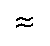
\includegraphics{almost_equals.eps}}
            ]
            \addplot+[mark=none, fill=blau_2a, draw = blau_2b] table[x=Pos, y=Avg, fill=red] {dataset};
            \legend{Stromverbrauch}
        \end{axis} 
        \begin{axis}[
            ybar,
            scale only axis,
            width = 0.85\textwidth,
            height = 0.5\textwidth,
            y axis line style=gruen_4b!100!black,
            axis y line* = right,
            axis x line = none,
            ylabel = Durchlaufszeit in mS,
            % height = 80mm,
            xmin = 0,
            xmax = 22,
            ymin = 0,
            xticklabel style={rotate=90},
            xticklabels from table = {dataset}{Name},
            xtick = {1,...,21},
            ymax = 246008,
            ymin = 109147,
            bar width = 2mm,
            bar shift = 1mm,
            legend style = {at={(0.5, 1.025)}, anchor = south west, legend columns = -1, draw=none, area legend},
            area legend,
            extra y ticks ={109147},
            extra y tick style = {grid=none, yticklabel style={yshift=2.5mm, xshift=-1.6mm, rotate=0, inner sep=.5pt}},
            extra y tick labels = {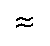
\includegraphics{almost_equals.eps}},
            ]
            \addplot+[mark=none,  fill=gruen_4a, draw = gruen_4b,] table[x=Pos, y=time] {dataset};
            \legend{Durchlaufszeit}
        \end{axis}
    \end{tikzpicture}
    \caption{Ausführung aller Benchmarks auf dem Galileo Board}
    \label{fig:benchmarks_galileo}
\end{figure}




%Vorlage fuer Thesen an der FFHS
\documentclass[class=minimal,border=0pt]{standalone}

\usepackage[utf8]{inputenc}

% addional configuration from sam
\usepackage{bibgerm}
\usepackage{hyperref}
\usepackage{cite}
\usepackage{etoolbox}
\usepackage{listings}
\usepackage{float}%
\usepackage{verbatim}
\usepackage{filecontents}
\usepackage{siunitx}
\sisetup{per=slash, load=abbr}
\usepackage{tikz}
\usepackage{pgfplots}
\pgfplotsset{width=7cm,compat=newest}
\usepackage[autostyle=true,german=quotes]{csquotes}
\usepackage{multirow}
\usepackage{hhline}
\usepackage{amsmath}
\RequirePackage{helvet}
\renewcommand{\familydefault}{\sfdefault}



\begin{document}

\input{../template/custom-colors.tex}


\begin{filecontents}{dataset}
Pos	Name	Bench1	Bench2	Bench3	time1	time2	time3	medbench	medtime	energymWh	power
1	nop	439	439.6	439.6	123555	123556	123556	439.6	123.556	77.8518118933	2.268336
2	nop\_nop	431.1	431.5	431.8	154444	154445	154445	431.5	154.445	95.5216584167	2.22654
3	nop\_nop\_nop	424.2	424.3	424.1	154447	154446	154446	424.2	154.446	93.90625692	2.188872
4	add\_0	435.3	435.5	435.5	123556	123556	123556	435.5	123.556	77.1257144667	2.24718
5	add\_32	438.4	438.6	438.7	108112	108112	108113	438.6	108.112	67.96568992	2.263176
6	sadd8\_0	429.3	429.5	429.5	123556	123555	123555	429.5	123.555	76.06251725	2.21622
7	sadd8\_8	437.7	437.6	437.6	123556	123555	123555	437.6	123.555	77.4969908	2.258016
8	sadd16\_0	434.9	434.7	434.9	123556	123556	123556	434.9	123.556	77.0194563067	2.244084
9	sadd16\_8	432.2	432.5	432.4	108112	108110	108112	432.4	108.112	67.0049346133	2.231184
10	sub\_0	435	434	434	123557	123555	123556	434	123.556	76.8600690667	2.23944
11	sub\_32	431.9	431.8	432.2	108111	108112	108112	431.9	108.112	66.9274543467	2.228604
12	lsr\_0	437.8	438	437.7	123556	123555	123555	437.8	123.555	77.5324099	2.259048
13	lsr\_32	438.6	438.8	438.7	108110	108112	108112	438.7	108.112	67.9811859733	2.263692
14	lsl\_0	438.5	438.7	438.7	108112	108112	108112	438.7	108.112	67.9811859733	2.263692
15	lsl\_32	429.8	429.8	430.2	123556	123556	123555	429.8	123.556	76.1162619467	2.217768
16	mul\_0	427.9	428.1	428.3	123558	123557	123557	428.1	123.557	75.81581077	2.208996
17	mul\_32	434.1	434.1	433.8	123559	123559	123560	434.1	123.559	76.87964539	2.239956
18	and\_0	434.7	434.9	435.2	123556	123554	123556	434.9	123.556	77.0194563067	2.244084
19	and\_32	438.5	438.6	438.5	108111	108112	108111	438.5	108.111	67.94956535	2.26266
20	or\_0	438.8	438.7	438.8	123555	123554	123554	438.8	123.554	77.7088764533	2.264208
21	or\_32	432.5	432.7	432.7	108112	108112	108113	432.7	108.112	67.0514227733	2.232732
22	xor\_0	429.4	429.4	429.3	123555	123555	123555	429.4	123.555	76.0448077	2.215704
23	xor\_32	432.2	432.5	432.6	108113	108112	108110	432.5	108.112	67.0204306667	2.2317
\end{filecontents}



    \begin{tikzpicture} 
        \begin{axis}[
            ybar,
            scale only axis,
            xlabel= Benchmarks,
            width = 1.5\textwidth,
            height = 0.5\textwidth,
            ylabel= Leistungsverbrauch in W,
            yticklabel style={/pgf/number format/fixed},
            y axis line style=blau_2b!100!black,
            % height = 80mm,
            ymin = 2.161872,
            ymax = 2.298336,
            xmin = 0,
            xmax = 24,
            bar width = 2mm,
            axis x line* = bottom,
            axis y line* = left,
            xticklabel style={rotate=90},
            xticklabels from table = {dataset}{Name},
            xtick = {1,...,23},
            bar shift = 0mm,
            legend style = {at={(0.5, 1.025)}, anchor = south east, legend columns = -1, draw=none, area legend},
            area legend,
            extra y ticks ={2.161872},
            extra y tick style = {grid=none, yticklabel style={yshift=2.5mm, xshift=1.9mm, rotate=0, inner sep=.5pt}},
            extra y tick labels = {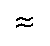
\includegraphics{almost_equals.eps}}
            ]
            \addplot+[mark=none, fill=blau_2a, draw = blau_2b] table[x=Pos, y=power, fill=red] {dataset};
            \legend{Leistungsverbrauch}
        \end{axis} 
        \begin{axis}[
            ybar,
            scale only axis,
            y axis line style=gruen_4b!100!black,
            width = 1.5\textwidth,
            height = 0.5\textwidth,
            axis y line* = right,
            axis x line = none,
            ylabel = Durchlaufszeit in S,
            % height = 80mm,
            xmin = 0,
            xmax = 24,
            ymin = 0,
            xticklabel style={rotate=90},
            xticklabels from table = {dataset}{Name},
            xtick = {1,...,23},
            ymax = 164.447,
            ymin = 92.112,
            bar width = 2mm,
            bar shift = 2mm,
            legend style = {at={(0.5, 1.025)}, anchor = south west, legend columns = -1, draw=none, area legend},
            area legend,
            extra y ticks ={92.112},
            extra y tick style = {grid=none, yticklabel style={yshift=2.5mm, xshift=-1.6mm, rotate=0, inner sep=.5pt}},
            extra y tick labels = {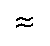
\includegraphics{almost_equals.eps}},
            ]
            \addplot+[mark=none,  fill=gruen_4a, draw = gruen_4b,] table[x=Pos, y=medtime] {dataset};
            \legend{Durchlaufszeit}
        \end{axis}


        \begin{axis}[
            ybar,
            at={(-20mm,0mm)},
            scale only axis,
            y axis line style=orange_6b!100!black,
            width = 1.5\textwidth,
            height = 0.5\textwidth,
            axis y line* = left,
            axis x line = bottom,
            ylabel = Energieverbrauch in m/Wh,
            % height = 80mm,
            xmin = 0,
            xmax = 24,
            ymin = 0,
            xticklabels = ,
            xtick = {0,...,23},
            xmajorticks=false,
            ymax = 100,
            ymin = 60,
            bar width = 2mm,
            bar shift = 18mm,
            legend style = {at={(0.25, 1.025)}, anchor = south west, legend columns = -1, draw=none, area legend},
            area legend,
            extra y ticks ={60},
            ytick = {65,70,...,100},
            extra y tick style = {grid=none, yticklabel style={yshift=2.5mm, xshift=2mm, rotate=0, inner sep=.5pt}},
            extra y tick labels = {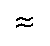
\includegraphics{almost_equals.eps}},
            ]
            \addplot+[mark=none,  fill=orange_6a, draw = orange_6b,] table[x=Pos, y=energymWh] {dataset};
            \legend{Energieverbrauch}
        \end{axis}



    \end{tikzpicture}





\end{document}





\section{Beobachtungen}

Betrachtet man die Durchlaufzeit wird klar ersichtlich, dass sie Stufen auf einer Ratioskala bilden. Die Intervalle können als CPU-Zyklen erklärt werden, wobei ein CPU-Zyklus immer gleich viel Zeit in Anspruch nimmt. Aus den Stufen, die die Durchlaufzeit wiedergibt, ist es möglich Zyklus-Kategorien zu bilden, je nachdem, ob ein Befehlssatz einen, zwei oder mehrere CPU-Zyklen durchläuft. Je nach Architektur des Prozessors und Komplexität des Befehlssatz benötigt die Abarbeitung mehrere CPU-Zyklen. Hinzu kommt, dass moderne Prozessoren fähig sind, mehrere Befehlssätze gleichzeitig auf einem einzelnen CPU-Kern (Single-Core) auszuführen. Dazu müssen jedoch sehr komplexe Voraussetzungen erfüllt sein, die vom Hersteller nicht immer gegeben sind.
\par
Wie bereits in \autoref{sec:auswertung_resultate} erläutert, ist der Energieverbrauch von den beiden Faktoren "Leistung" und "Zeit" abhängig. Dabei wirkt sich die Zeit gravierender auf den Energieverbrauch der Benchmarks aus als die Leistung. Wie aus den Abbildungen \autoref{fig:benchmarks_galileo} und \ref{fig:benchmarks_rasp} ersichtlich, sind die Leistungsunterschiede innerhalb einer Zyklus-Kategorie minim im Gegensatz zu einer höheren Zyklus-Kategorie. Multipliziert man die Leistungsverbrauche der unterschiedlichen Zyklus-Kategorien mit ihren jeweiligen Durchlaufszeiten, werden die Differenzen im Verbrauch jedoch markanter. Somit ist erwiesen, dass der Faktor "Zeit" den grösseren Einfluss auf den Stromverbrauch ausübt. 
\par
Innerhalb ähnlicher Zyklus-Kategorien können durchaus Leistungsunterschiede gemessen werden, wie dies beispielsweise die Daten vom Raspberry Pi Board \texttt{add\_0} und \texttt{add\_32} oder vom Galileo Board \texttt{addl\_0} und \texttt{addl\_32} darlegen. Daraus geht hervor, dass das Galileo Board bei der Addition von grösseren Zahlen einen höheren Leistungsverbrauch hat als bei der von kleineren. Beim Raspberry Pi Board stellt sich die Situation gerade umgekehrt dar. Um die Ursache dieses Phänomens zu finden, müssten an dieser Stelle weitere Forschungen angestrebt werden.
\par
Wird der Fokus auf die beiden Benchmarks \texttt{sadd16\_8} und \texttt{add\_32} gelegt, die auf dem Raspberry Pi Board ausgeführt werden, ergibt sich die folgende Erkenntnis: Die Additionsoperation, die parallel zwei Mal eine Zahl von 16bit rechnen kann, nimmt weniger Leistung in Anspruch als die Additionsoperation einer 32bit-Zahl. Könnte also für Zahlen bis zu einer Grösse von 16bit konsequent die Assemblerinstruktion \texttt{sadd16} anstelle von \texttt{add} gewählt werden, ergäbe sich womöglich ein Sparpotenzial. Die beiden Benchmarks haben einen Verbrauch von 2.231W und 2.263W\footnote{Vgl. im Anhang Kap. 1.2}. Das Ersparnispotenzial betrüge somit also 32mW oder zirka 1.4 Prozent. Dabei ist aber zu bedenken, dass die Energieersparnis erst nach 21 Milliarden Durchläufen eintritt. Diese sind je nach Art der Anwendung allerdings relativ schnell erreicht. Als Beispiel ist hier an die Pixelberechnung eines Bildes zu denken.


















\chapter{Fazit}
\section{Diskussion}
%Vergleich mit ähnliche Papers (z.B. Energiemessung durch thermische Kamera)
Das Resultat in Sätze gefasst



\input{sections/selbsterklaerung}


%\begin{thebibliography}{1}
%\end{thebibliography}
\bibliography{thesis_bibliography}
\bibliographystyle{gerplain}
\listoffigures



\end{document}


